%%% LaTeX Template: Article/Thesis/etc. with colored headings and special fonts
%%%
%%% Source: http://www.howtotex.com/
%%% Feel free to distribute this template, but please keep to referal to http://www.howtotex.com/ here.
%%% February 2011
%%%
%%% Modified January 2016 by CDM

%%%  Preamble
\documentclass[11pt,letterpaper]{article}
\usepackage[margin=1.0in]{geometry}
\usepackage[T1]{fontenc}
\usepackage[bitstream-charter]{mathdesign}
\usepackage[latin1]{inputenc}					
\usepackage{amsmath}						
\usepackage{xcolor}
\usepackage{cite}
\usepackage{hyphenat}
\usepackage{graphicx}
\usepackage{float}
\usepackage{subfigure}
\usepackage{sectsty}
\usepackage[compact]{titlesec} 
\usepackage[tablegrid]{vhistory}
\usepackage{pbox}
\allsectionsfont{\color{accentcolor}\scshape\selectfont}

%%% Definitions
\definecolor{accentcolor}{rgb}{0.0,0.0,0.5} 
\newcommand{\teamname}{Team Name}
\newcommand{\productname}{Product Name}
\newcommand{\coursename}{CSE 4316: Senior Design I}
\newcommand{\semester}{Fall 2015}
\newcommand{\docname}{Architectural Design Specification}
\newcommand{\department}{Department of Computer Science \& Engineering}
\newcommand{\university}{The University of Texas at Arlington}
\newcommand{\authors}{Alan Turing \\ Grace Hopper \\ John Von Neumann \\ Ada Lovelace \\ Charles Babbage}

%%% Headers and footers
\usepackage{fancyhdr}
	\pagestyle{fancy}						% Enabling the custom headers/footers
\usepackage{lastpage}	
	% Header (empty)
	\lhead{}
	\chead{}
	\rhead{}
	% Footer
	\lfoot{\footnotesize \teamname \ - \semester}
	\cfoot{}
	\rfoot{\footnotesize page \thepage\ of \pageref{LastPage}}	% "Page 1 of 2"
	\renewcommand{\headrulewidth}{0.0pt}
	\renewcommand{\footrulewidth}{0.4pt}

%%% Change the abstract environment
\usepackage[runin]{abstract}			% runin option for a run-in title
%\setlength\absleftindent{30pt}			% left margin
%\setlength\absrightindent{30pt}		% right margin
\abslabeldelim{\quad}	
\setlength{\abstitleskip}{-10pt}
\renewcommand{\abstractname}{}
\renewcommand{\abstracttextfont}{\color{accentcolor} \small \slshape}	% slanted text

%%% Start of the document
\begin{document}

%%% Cover sheet
{\centering \huge \color{accentcolor} \sc \textbf{\department \\ \university} \par}
\vspace{1 in}
{\centering \huge \color{accentcolor} \sc \textbf{\docname \\ \coursename \\ \semester} \par}
\vspace{0.5 in}
\begin{figure}[h!]
	\centering
   	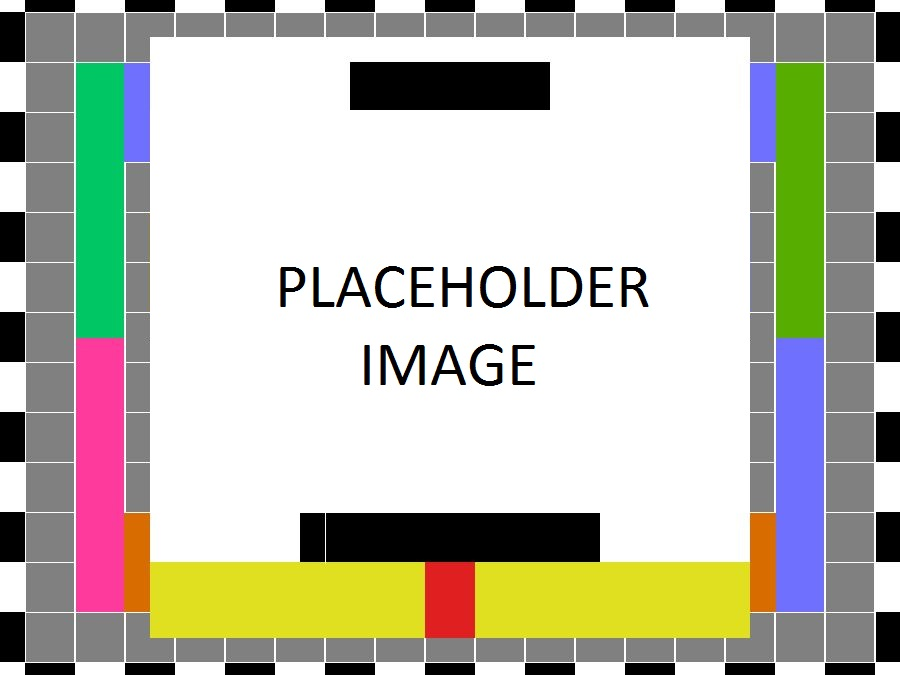
\includegraphics[width=0.60\textwidth]{images/test_image}
\end{figure}
\vspace{0.5 in}
{\centering \huge \color{accentcolor} \sc \textbf{\teamname \\ \productname} \par}
\vspace{0.5 in}
{\centering \large \sc \textbf{\authors} \par}
\newpage


%\vspace{1 in}
%\centerline{January 13th, 2012}
%\newpage

%%% Revision History
\begin{versionhistory}
  	\vhEntry{0.1}{10.01.2015}{GH}{document creation}
  	\vhEntry{0.2}{10.05.2015}{AT|GH}{complete draft}
  	\vhEntry{0.3}{10.12.2015}{AT|GH}{release candidate 1}
  	\vhEntry{1.0}{10.20.2015}{AT|GH|CB}{official release}
  	\vhEntry{1.1}{10.31.2015}{AL}{added design review requests}
\end{versionhistory}
\newpage

%%% Table of contents
\setcounter{tocdepth}{2}
\tableofcontents
\newpage

%%% List of figures and tables (optional)
\listoffigures
\listoftables
\newpage

%%% Document sections
\section{Introduction}
The Turing Board is a concept autonomous longboard which is capable of exhibiting self-driving capabilities using computer vision. Users of the Turing Board will be able to take advantage of various features such as having the board follow you autonomously and having the board summon itself to you from a parked location, in addition to functioning as a standard electric longboard capable of recording and analyzing all trip data. Users will also be able to use the Turing Board to function as a load carrier, relieving them from the burden of carrying everyday items like backpacks, boxes, etc. if desired. 
The main components of the Turing Board include a remote control via an app on the user's phone, the Jetson TX2 controlling the software signals and output to other components of the board, the motorized wheels and turning mechanism, computer vision, human-machine interface, and the board's power supply. 

\newpage
\section{System Overview}
This section should describe the overall structure of your software system. Think of it as the strategy for how you will build the system. An architectural "layer" is the top-level logical view, or an abstraction, of your design. Layers should be composed of related elements of similar capabilities, and should be highly independent of other layers, but should have very clearly defined interfaces and interactions with other layers. Each layer should be identified individually and should be unique as to its function and purpose within the system. This section should also contain the high-level block diagram of the layers, as shown in the example below, as well as detailed descriptions of the functions of each layer.

\begin{figure}[h!]
	\centering
 	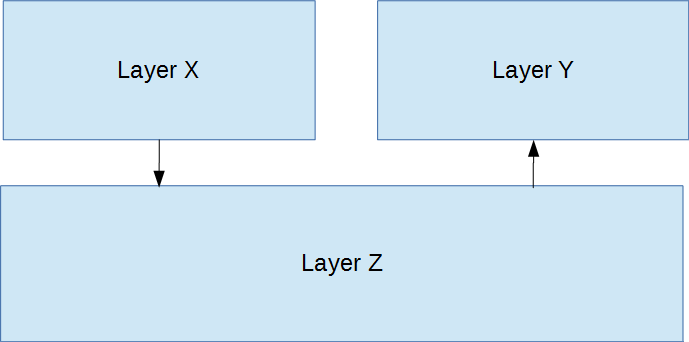
\includegraphics[width=0.60\textwidth]{images/layers}
 \caption{A simple architectural layer diagram}
\end{figure}

\subsection{Computer Vision Layer}
This layer is the heart of the core autonomous functionalities of the Turing Board. We use computer vision and depth imagery to determine the board's surroundings and calculate the best path to move forward. The user will have, strapped around their ankle, an elastic band affixed with a pattern of ArUco markers for the \textit{Follow Along} feature. This layer tracks the movement of the user vis-a-vis the anklet to determine how to instruct the combination of motors to move so as to follow the user at an appropriate pace. It is also responsible for detecting possible obstacles when operating on its own to find the user as part of the \textit{Summon} feature. 
Data taken in from the cameras will flow from this layer into the Main Control Layer to be processed and then send out the appropriate signals primarily to the Wheels \& Turning Layer. This layer also takes in data from the anklet component in the HMI layer specifically for the Follow feature.

\subsection{Remote Control Layer}
This layer is controlled directly by the user. It takes the form of an app that sends data to the Main Control layer for the appropriate signals to be sent to the other layers. The app requires an authentication process to log into it. It will also provide the user with ride data analysis after a trip on the board is completed. This app is available on iOS and Android.

\subsection{Power Layer}
This layer is responsible for controlling the power distributed to the electrical components on the Turing Board. It directly powers portions of both the HMI layer and the Wheels \& Turning layer. This layer ensures power is not over-distributed by way of a Buck converter. It also provides data on how much charge is left in the battery at any given time. This data is sent to the Main Controls layer for the appropriate signals to be sent out to the other layers as needed.

\subsection{Main Controls Layer}
This layer is in charge of processing and sending out the majority of the signals on the Turning Board. It receives data from the Computer Vision layer, the Remote Control Layer, and the Power layer. With these inputs, it sends data to the HMI layer as well as the Wheels \& Turning layer. The Jetson TX2 provides the computing power in this layer and will process all of these needs. It will also fetch data from a real-time database and directly interact with a separate micro-controller that is in charge of the minor systems on the Turing Board.

\subsection{HMI Layer}
This layer contains all of the hardware parts of the Turing Board that interacts directly with the user. This layer includes LEDs, a pressure sensor, a buzzer/speaker, and an anklet. The LEDs let the user know what mode the board is in (Summon, Follow, or Electric) based off of the color they are emitting at the time. The pressure sensor determines how much weight is currently on the board and transmits this information to the Main Controls layer to control what mode the board is in. The buzzer or speaker will make a sound if the user steps onto the board when it is not in Electric mode to notify them of improper usage. Finally, the anklet is to be worn by the user to give data to the Computer Vision layer when the board is in Follow mode.

\subsection{Wheels \& Turning Layer}
This layer contains the components needed to cause the board to move and turn. It contains the ESC, brushless motors, stepper motors, optical sensors for the stepper motors, solenoids, optical sensors for the solenoids, the micro-controller, and the turning mechanism. The ESC will control the speed at which the brushless motors inside of the wheels turn as determined by signals sent from the Main Controls layer. The stepper motor will turn the turning mechanism a certain amount of degrees not exceeding 30-45 in either direction as determined by the Main Controls layer. The optical sensor for the stepper motor will track how many degrees the turning mechanism has been turned and send this data to the Main Controls layer. The solenoids will be responsible for locking the turning mechanism in place when it is in Electric mode. The optical sensors for the solenoids will determine if the solenoids are properly locked in place or not and transmit this data to the Main Controls layer. The micro-controller will receive data from the Main Controls layer and use that to output the necessary signals to the motors. 


\newpage
\section{Subsystem Definitions \& Data Flow}
This section breaks down your layer abstraction to another level of detail. Here you grapically represent the logical subsytems that compose each layer and show the interactions/interfaces between those subsystems. A subsystem can be thought of as a programming unit that implements one of the major functions of the layer. It, therefore, has data elements that serve as source/sinks for other subsystems. The logical data elements that flow between subsystems need to be explicitly defined at this point, beginning with a data flow-like diagram based on the block diagram.

\begin{figure}[h!]
	\centering
 	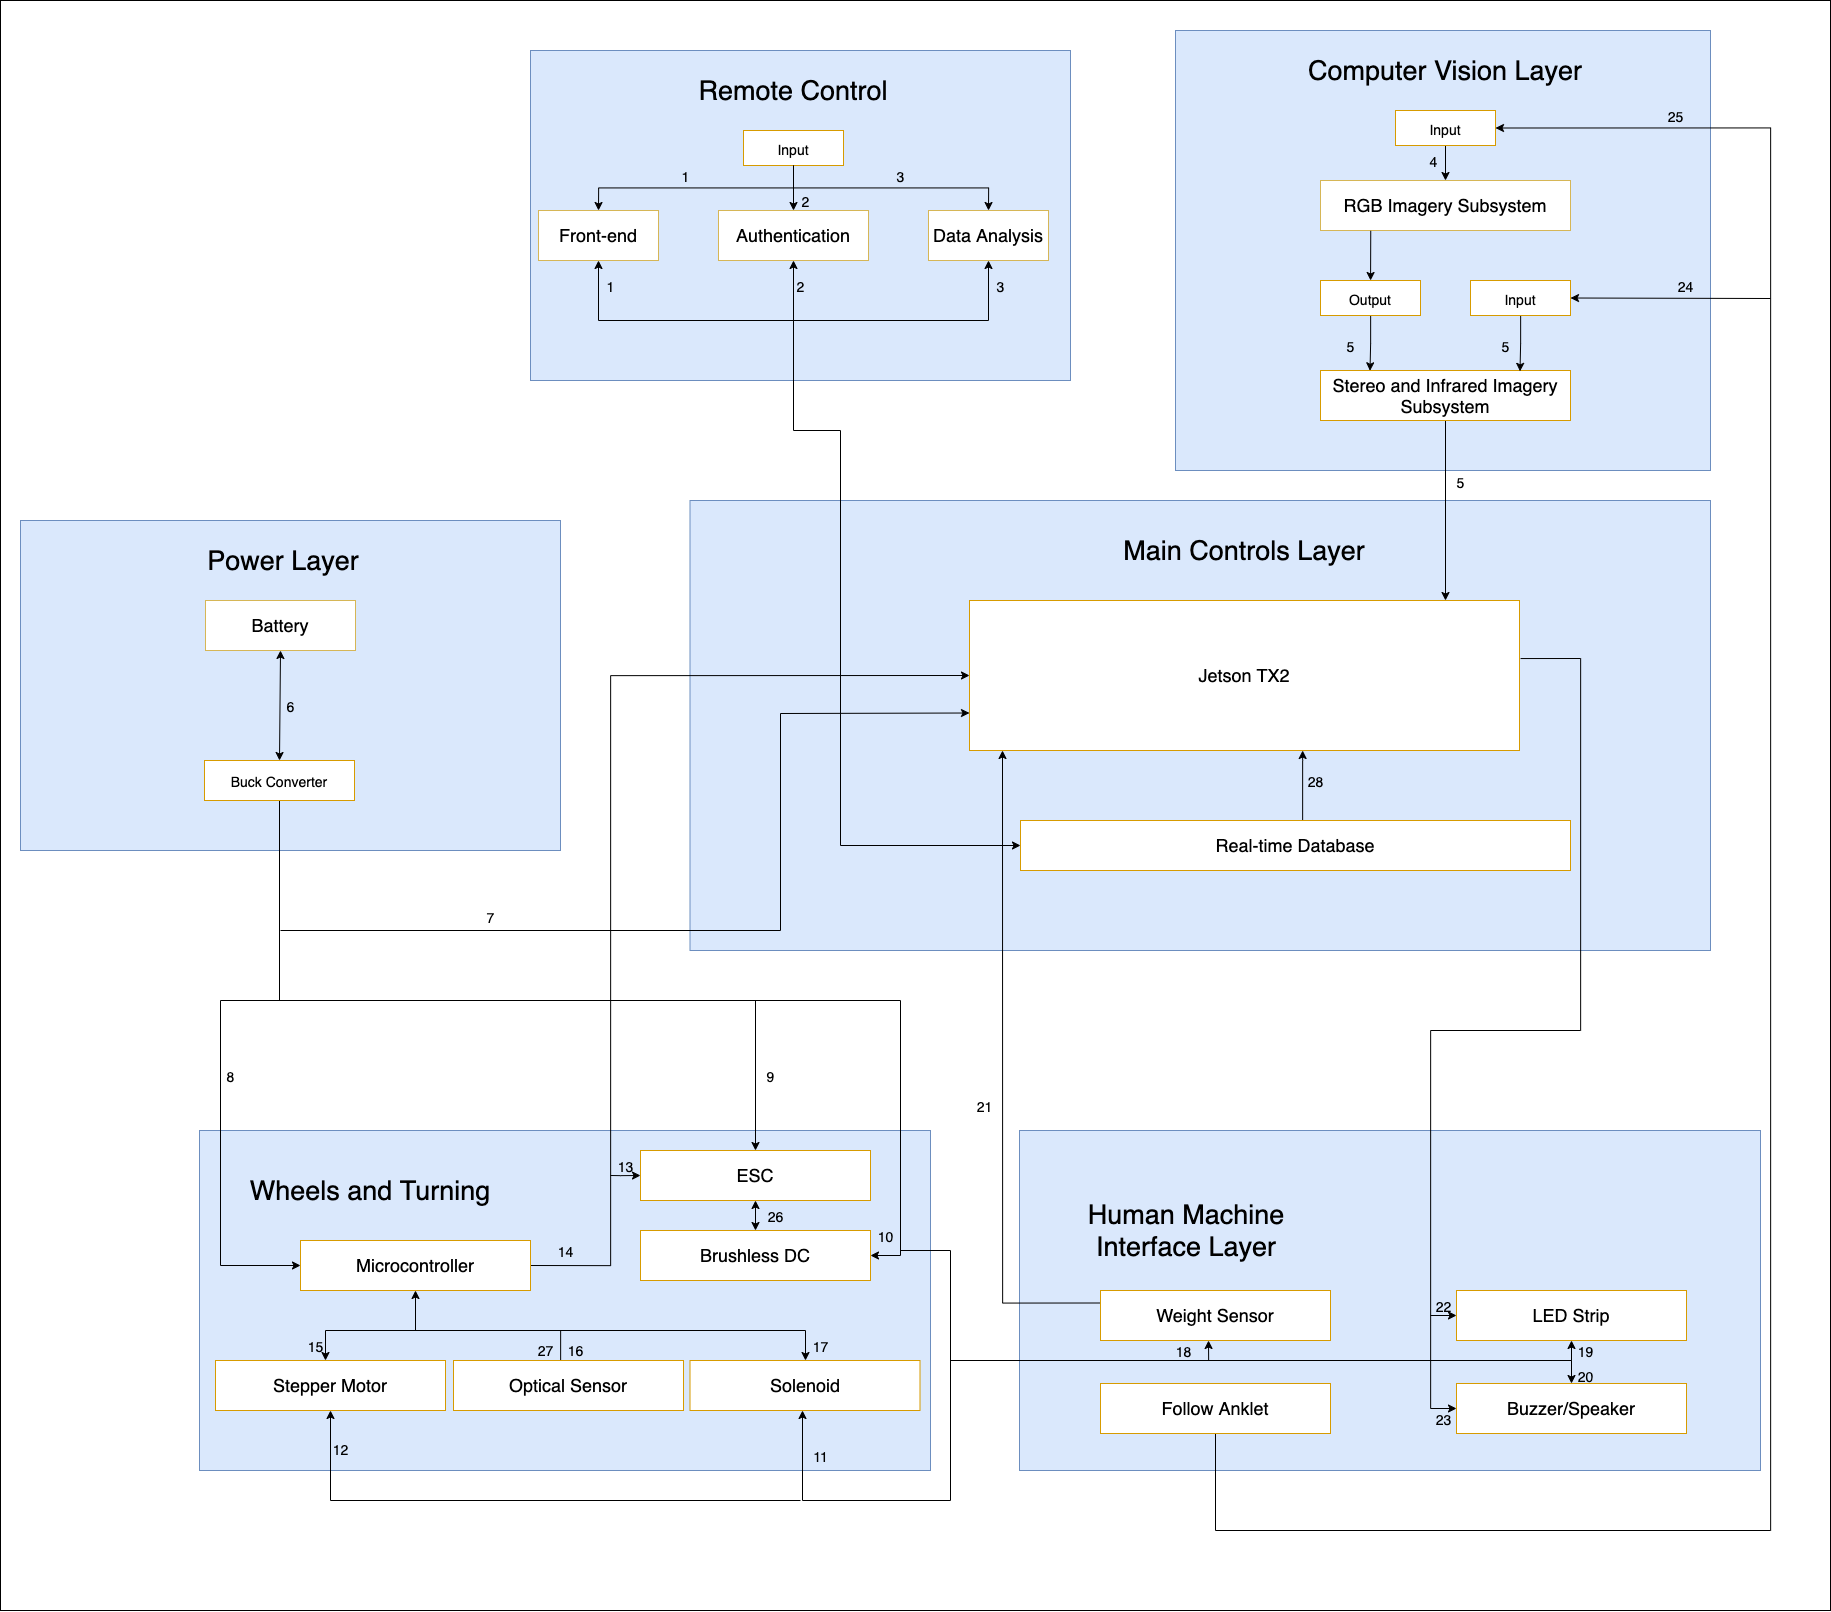
\includegraphics[width=\textwidth]{images/data_flow}
 \caption{A simple data flow diagram}
\end{figure}

\newpage
\section{X Layer Subsystems}
In this section, the layer is described in some detail in terms of its specific subsystems. Describe each of the layers and its subsystems in a separate chapter/major subsection of this document. The content of each subsystem description should be similar. Include in this section any special considerations and/or trade-offs considered for the approach you have chosen.

\subsection{Subsystem 1}
This section should be a general description of a particular subsystem for the given layer. For most subsystems, an extract of the architectural block diagram with data flows is useful. This should consist of the subsystem being described and those subsystems with which it communicates.

\begin{figure}[h!]
	\centering
 	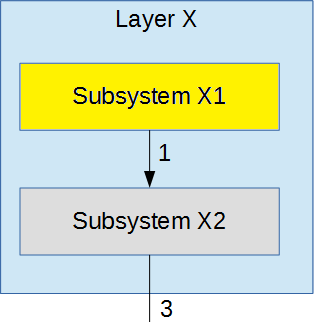
\includegraphics[width=0.60\textwidth]{images/subsystem}
 \caption{Example subsystem description diagram}
\end{figure}

\subsubsection{Assumptions}
Any assumptions made in the definition of the subsystem should be listed and described. Pay particular attention to assumptions concerning interfaces and interactions with other layers.

\subsubsection{Responsibilities}
Each of the responsibilities/features/functions/services of the subsystem as identified in the architectural summary must be expanded to more detailed responsibilities. These responsibilities form the basis for the identification of the finer-grained responsibilities of the layer's internal subsystems. Clearly describe what each subsystem does.

\subsubsection{Subsystem Interfaces}
Each of the inputs and outputs for the subsystem are defined here. Create a table with an entry for each labelled interface that connects to this subsystem. For each entry, describe any incoming and outgoing data elements will pass through this interface.

\begin {table}[H]
\caption {Subsystem interfaces} 
\begin{center}
    \begin{tabular}{ | p{1cm} | p{6cm} | p{3cm} | p{3cm} |}
    \hline
    ID & Description & Inputs & Outputs \\ \hline
    \#xx & Description of the interface/bus & \pbox{3cm}{input 1 \\ input 2} & \pbox{3cm}{output 1}  \\ \hline
    \#xx & Description of the interface/bus & \pbox{3cm}{N/A} & \pbox{3cm}{output 1}  \\ \hline
    \end{tabular}
\end{center}
\end{table}

\subsection{Subsystem 2}
Repeat for each subsystem

\subsection{Subsystem 3}
Repeat for each subsystem


\newpage
\section{Controls Software Layer}
This layer is responsible for binding all modules of the Turing Board into one cohesive system. All data coming in is intercepted by this layer and forwarded to the respective modules, which are responsible for processing the forwarded data.

\subsection{Data Processing}
There are three main components of the project which requires this piece of software and must all be non-blocking in nature to ensure the entire system stays responsive.
\begin{itemize}
    \item Reading data from the micro-controller.
    \item Forwarding data to the micro-controller.
    \item Fetching data from the Firebase Real-time database.
\end{itemize}

\begin{figure}[h!]
	\centering
 	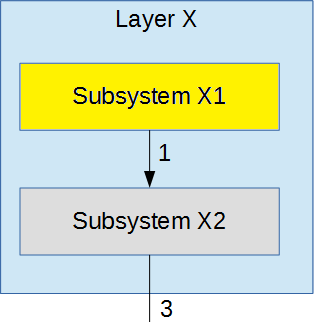
\includegraphics[width=0.60\textwidth]{images/subsystem}
 \caption{Example subsystem description diagram}
\end{figure}

\subsubsection{Assumptions}
The user of the Turing Board is assumed to always be connected to a network (and access the World Wide Web) to ensure data can be received from the database and forwarded to the wheels.

\subsubsection{Responsibilities}
After fetching data from the database, the controls software will first process the data to an extent. Since incoming data will be floating point values, it first needs to be translated into a value which the micro-controller can understand. Thus, the entire range of data is relayed from the remote control app and the required data is then mapped from 0-255, which is then forwarded to the micro-controller. This, in turn, causes the wheels to change speed as needed. As part of the same data packet, angle data from the controls code is also sent to the micro-controller, which aids in rotating the turning mechanism to a specific angle with respect to the origin (0 degrees). Any data, such as weight values for someone who is standing on the longboard (an integral part of the design so that the software knows when to turn off the turning mechanism) is received back in the same data format (0-255), which then gets translated to weight values inside of the controls code.

\subsubsection{Subsystem Interfaces}
Each of the inputs and outputs for the subsystem are defined here.

\begin {table}[H]
\caption {Controls Software Interfaces} 
\begin{center}
    \begin{tabular}{ | p{1cm} | p{5cm} | p{3cm} | p{5cm} |}
    \hline
    ID & Description & Inputs & Outputs \\ \hline
    \#1 & Data Fetching \& Wheel Velocity Control & \pbox{3cm}{Speed Value} & \pbox{5cm}{Change Wheel Velocity}  \\ \hline
    \#2 & Controlling Turning Mechanism & \pbox{3cm}{Angle Value \\ Weight Value} & \pbox{5cm}{Rotates the Turning Mechanism \\ Toggles Turning Mechanism (On/Off)}  \\ \hline
    \end{tabular}
\end{center}
\end{table}
\newpage
\section{Power Delivery Layer}
In this section, the layer is described in some detail in terms of its specific subsystems. Describe each of the layers and its subsystems in a separate chapter/major subsection of this document. The content of each subsystem description should be similar. Include in this section any special considerations and/or trade-offs considered for the approach you have chosen.

\subsection{Subsystem 1}
This section should be a general description of a particular subsystem for the given layer. For most subsystems, an extract of the architectural block diagram with data flows is useful. This should consist of the subsystem being described and those subsystems with which it communicates.

\begin{figure}[h!]
	\centering
 	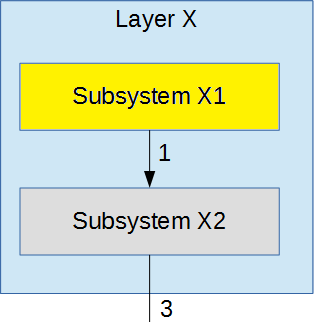
\includegraphics[width=0.60\textwidth]{images/subsystem}
 \caption{Example subsystem description diagram}
\end{figure}

\subsubsection{Assumptions}
Any assumptions made in the definition of the subsystem should be listed and described. Pay particular attention to assumptions concerning interfaces and interactions with other layers.

\subsubsection{Responsibilities}
Each of the responsibilities/features/functions/services of the subsystem as identified in the architectural summary must be expanded to more detailed responsibilities. These responsibilities form the basis for the identification of the finer-grained responsibilities of the layer's internal subsystems. Clearly describe what each subsystem does.

\subsubsection{Subsystem Interfaces}
Each of the inputs and outputs for the subsystem are defined here. Create a table with an entry for each labelled interface that connects to this subsystem. For each entry, describe any incoming and outgoing data elements will pass through this interface.

\begin {table}[H]
\caption {Subsystem interfaces} 
\begin{center}
    \begin{tabular}{ | p{1cm} | p{6cm} | p{3cm} | p{3cm} |}
    \hline
    ID & Description & Inputs & Outputs \\ \hline
    \#xx & Description of the interface/bus & \pbox{3cm}{input 1 \\ input 2} & \pbox{3cm}{output 1}  \\ \hline
    \#xx & Description of the interface/bus & \pbox{3cm}{N/A} & \pbox{3cm}{output 1}  \\ \hline
    \end{tabular}
\end{center}
\end{table}

\subsection{Subsystem 2}
Repeat for each subsystem

\subsection{Subsystem 3}
Repeat for each subsystem


\newpage

%%% References
\bibliographystyle{plain}
\bibliographystyle{reference/IEEEtran_custom}
\bibliography{reference/refs}{}

\end{document}